\section{Gravitationele Tijdsdilatatie}

In de algemene relativiteitstheorie lopen klokken dieper in een gravitationele potentiaalput langzamer vergeleken met klokken met hogere potentialen. We reproduceren dit resultaat met behulp van ætherstroomvelden in plaats van ruimtetijdkromming.

\subsection*{Ætherstroom als zwaartekracht}

We nemen aan dat massa $M$ een inwaartse radiale stroming van æther induceert. Bij een straal $r$ wordt deze stroomsnelheid gegeven door:
\[
    v_g(r) = \sqrt{\frac{2GM}{r}}.
\]


\begin{figure}[htbp]
    \centering
    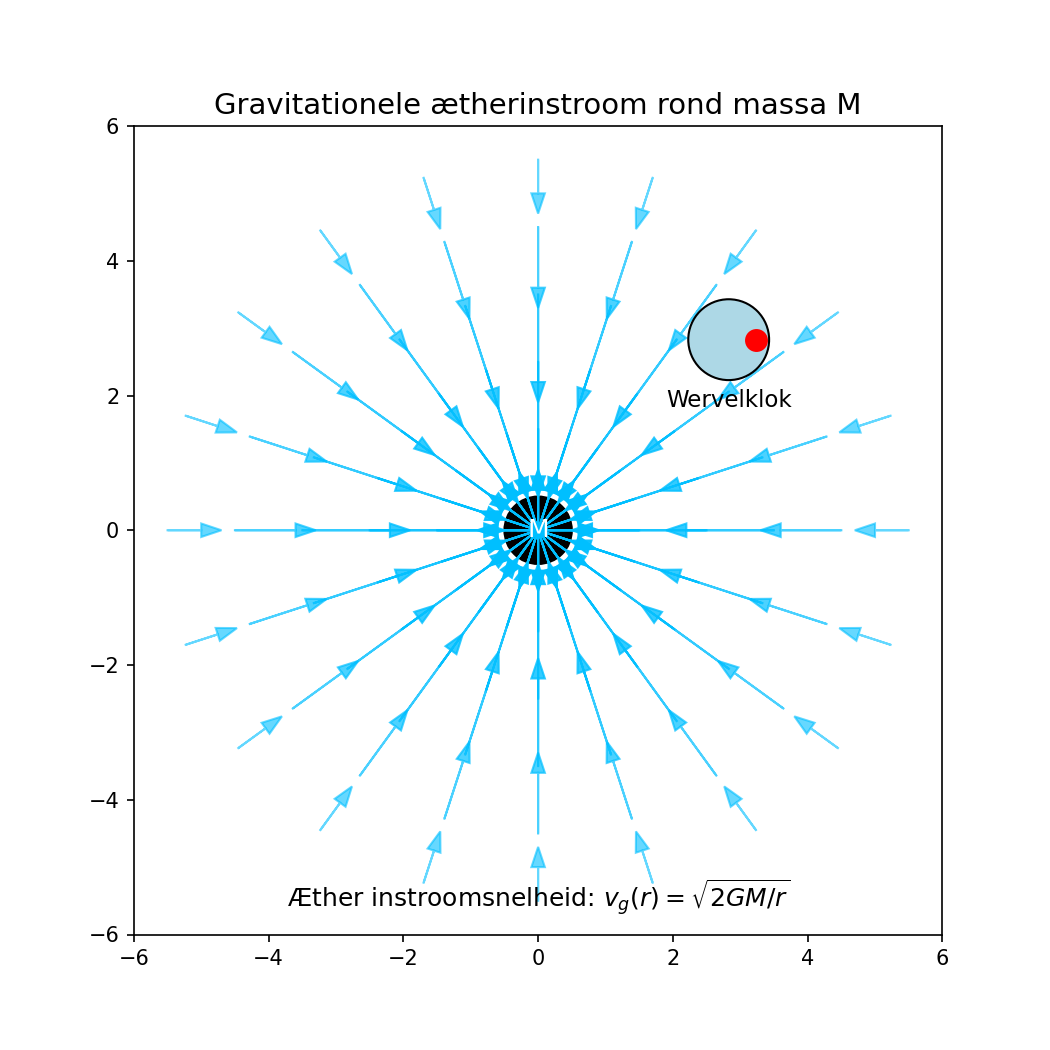
\includegraphics[width=0.85\textwidth]{07-GravitationeleÆtherinstroom}
    \caption{Gravitationele tijdsdilatatie door radiale ætherinstroom richting een massa~$M$. De wervelklok ervaart een lagere hoeksnelheid door ætherweerstand, analoog aan de Schwarzschild-roodverschuiving.}
    \label{fig:GravitationeleÆtherinstroom}
\end{figure}

Dit weerspiegelt de Painlevé-Gullstrand-metriek en het riviermodel van zwarte gaten~\cite{Hamilton2004-river}.

\subsection*{Ætherweerstand en klokvertraging}

Een klok die op straal $r$ in deze inwaartse ætherstroom wordt gehouden, ziet æther er langs bewegen met snelheid $v_g(r)$. De waargenomen hoeksnelheid van de wervelkern wordt daarom verminderd door de weerstand van de æther, net als in het speciale relativiteitsgeval, waarbij beweging door de æther de waargenomen kloksnelheid vermindert.

De gravitationele tijdsdilatatiefactor is dus:
\[
    \frac{d\tau}{dt} = \sqrt{1 - \frac{v_g^2(r)}{c^2}} = \sqrt{1 - \frac{2GM}{rc^2}}. \tag{4}
\]
Dit komt overeen met de Schwarzschild-oplossing voor stationaire waarnemers in de algemene relativiteitstheorie.

Een nauwkeurige bevestiging van gravitationele tijdsdilatatie onder gecontroleerde omstandigheden werd geleverd door de Gravity Probe A-missie~\cite{vessot_levine_1980}, waarbij een waterstofklok werd gelanceerd tot 10.000 km hoogte.

Deze vertraging is niet alleen theoretisch afgeleid, maar werd experimenteel bevestigd door Pound en Rebka in 1959, die met behulp van het Mössbauer-effect een gravitationeel veroorzaakte frequentieverschuiving maten tussen twee punten op verschillende hoogten binnen het zwaartekrachtsveld van de aarde~\cite{pound_rebka_1959}.


\subsection*{Interpretatie}

Deze vergelijking betekent dat hoe dieper een wervel zich in het gravitatiepotentieel bevindt (hoe sneller de lokale ætherstroom), hoe langzamer deze roteert vanuit het perspectief van een waarnemer op oneindig. Bij de Schwarzschild-straal $r_s = 2GM/c^2$, $d\tau/dt = 0$: de tijd stopt voor externe waarnemers.

Dit levert een mechanistische interpretatie van gravitationele roodverschuiving op: licht dat wordt uitgezonden door een wervelklok in een sterke potentiaalput, lijkt roodverschoven vanwege de langzamere hoekbeweging van de uitzendende wervel. Het resultaat:
\[
    \boxed{\frac{d\tau}{dt} = \sqrt{1 - \frac{2GM}{rc^2}}}
\]
is volledig consistent met GR en ondersteunt de æther-stroomanalogie~\cite{Schiller2022-maxforce}.